\documentclass[a4paper, 12pt]{article}

\usepackage{wrapfig}
\usepackage{graphicx}
\usepackage{mathtext}
\usepackage{amsmath}
\usepackage{siunitx} % Required for alignment
\usepackage{multirow}
\usepackage{rotating}
\usepackage{float}

\usepackage[T1,T2A]{fontenc}
\usepackage[russian]{babel}

\graphicspath{{pictures/}}

\title{\begin{center}Лабораторная работа №1.1.4\end{center}
Измерение интенсивности радиационного фона}
\author{Габорак Александр Витальевич \\ Б02-203}
\date{\today}

\begin{document}
    \pagenumbering{gobble}
    \maketitle
    \newpage
    \pagenumbering{arabic}

    \section{Введение}
    \textbf{Цель работы:}
    \begin{itemize}
        \item Применить методы обработки экспериментальных данных для изучения статистических закономерностей при измерении интенсивности радиационного фона
    \end{itemize}

    \vspace{1cm}

    \textbf{В работе используются: }
    \begin{itemize}
        \item счетчик Гейгера-Мюллера
        \item блок питания
        \item компьютер с интерфейсом связи со счетчиком

    \end{itemize}

    \section{Ход работы}
    \paragraph{}
    Проведем измерение используя интерфейс компьютера. Приведем данные в таблицу и начнем  обработку. Разбивая данные для 20 с по парам и просуммировав пары получим данные для 40 с.
    \paragraph{}
    Проверим связь $\sigma_{отд}\approx \sqrt{\bar{n}}$. Индекс 1 для 10 с, 2 для 40 с
    \[n_{общ} = \sum n_i = 5671\]
    \[\bar{n}_1 = \frac{n_{общ}}{N_1} = 14.1775\]
    \[\bar{n}_2 = \frac{n_{общ}}{N_2} = 56.71\]
    \[\sigma_{1}=\sqrt{\frac{1}{N_1} \sum_{i=1}^{N_1} (n_i - \bar{n}_i)^2} \approx 3.83\]
    \[\sigma_{2}=\sqrt{\frac{1}{N_2} \sum_{i=1}^{N_2} (n_i - \bar{n}_i)^2} \approx 7.73\]
    \newpage

    \[\sqrt{\bar{n}_1} =3.76 \approx 3.83 = \sigma_1\]
    \[\sqrt{\bar{n}_2} =7.53 \approx 7.73 = \sigma_2\]
    \paragraph{}
    Как видим связь между среднеквадратическим отклонением и среднем значении есть $(\sigma \approx \sqrt{\bar{n}})$.
    Теперь определим долю случаев в пределах $\pm\sigma$ и $\pm2\sigma$.

    \begin{table}[H]
    \begin{center}
    \begin{tabular}{|c|c|c|c|}\hline
    \multicolumn{4}{|c|}{$t=10с$}\\\hline
    Предел & Число случаев & Доля случаев & Теоретическая оценка\\\hline
    $\pm \sigma_1 = \pm 3.8$ & 281 & 70\% & 68\% \\
    $\pm 2\sigma_1 = \pm 7.7$ & 385 & 96\% & 95\% \\\hline
    \multicolumn{4}{c}{}\\\hline
    \multicolumn{4}{|c|}{$t=10с$}\\\hline
    Предел & Число случаев & Доля случаев & Теоретическая оценка\\\hline
    $\pm \sigma_2 = \pm 7.7$ & 68 & 68\% & 68\% \\
    $\pm 2\sigma_2 = \pm 15.5$ & 93 & 93\% & 95\% \\\hline

    \end{tabular}
    \caption{Количество измерении за пределами $\pm\sigma$ и $\pm2\sigma$}
    \end{center}
    \end{table}

    \paragraph{}
    Как видим наши данные с довольно хорошей точностью соответствуют теории. Как видно из графика относительный разброс данных за 40с меньше чем за 10с. Подсчитаем какая разница между этими 2мя случаями.
    \[\frac{\sigma_1}{\bar{n}_1} \approx 27\%, \frac{\sigma_2}{\bar{n}_2} \approx 14\%\]
    \paragraph{}
    Как видим разница почти в 2 раза, что и следует от того факта что $\sigma \approx \sqrt{\bar{n}}$.
    \paragraph{}
    Для финального ответа подсчитаем ошибки средних величин. По теории
    \[\sigma_{\bar{n}_1} = \frac{\sigma_{1}}{N_1} \approx 0.19, \sigma_{\bar{n}_2} \approx 0.77\]
    \[\varepsilon_{\bar{n}_1} = \frac{\sigma_{\bar{n}_1}}{\bar{n}_1}\approx 1.3\%, \varepsilon_{\bar{n}_2}\approx 1.3\%\]
    Получаем финальный результат
    \[n_{t=10с}=14.17 \pm 0.19\]
    \[n_{t=40с}=56.71 \pm 0.77\]

    \newpage
    \begin{table}[H]
    \begin{center}
    \begin{tabular}{|c|r|r|r|r|r|r|r|r|r|r|}
    \hline
    {№ опыта} &   1 &   2 &   3 &   4 &   5 &   6 &   7 &   8 &   9 &  10 \\
    \hline
    0   &  38 &  24 &  45 &  26 &  33 &  21 &  30 &  21 &  26 &  18 \\
    10  &  27 &  33 &  32 &  36 &  31 &  26 &  36 &  16 &  25 &  23 \\
    20  &  29 &  32 &  27 &  28 &  29 &  27 &  29 &  30 &  27 &  28 \\
    30  &  19 &  29 &  26 &  26 &  20 &  21 &  34 &  31 &  30 &  30 \\
    40  &  31 &  28 &  24 &  29 &  21 &  21 &  28 &  29 &  25 &  29 \\
    50  &  29 &  33 &  20 &  31 &  31 &  26 &  40 &  22 &  28 &  24 \\
    60  &  18 &  48 &  19 &  33 &  35 &  31 &  21 &  34 &  26 &  32 \\
    70  &  23 &  27 &  33 &  40 &  28 &  36 &  32 &  40 &  31 &  24 \\
    80  &  24 &  30 &  26 &  22 &  31 &  42 &  27 &  40 &  34 &  26 \\
    90  &  29 &  25 &  25 &  32 &  25 &  29 &  23 &  33 &  23 &  28 \\
    100 &  30 &  27 &  37 &  36 &  31 &  28 &  28 &  35 &  28 &  33 \\
    110 &  22 &  35 &  28 &  32 &  39 &  32 &  28 &  15 &  24 &  22 \\
    120 &  34 &  21 &  21 &  26 &  28 &  32 &  22 &  25 &  31 &  26 \\
    130 &  20 &  39 &  30 &  21 &  16 &  25 &  28 &  22 &  28 &  26 \\
    140 &  17 &  22 &  28 &  27 &  25 &  34 &  34 &  28 &  27 &  39 \\
    150 &  25 &  28 &  28 &  28 &  28 &  35 &  32 &  28 &  27 &  28 \\
    160 &  27 &  19 &  26 &  35 &  29 &  23 &  31 &  28 &  23 &  33 \\
    170 &  30 &  26 &  34 &  31 &  40 &  35 &  22 &  28 &  22 &  26 \\
    180 &  23 &  30 &  29 &  32 &  38 &  31 &  24 &  25 &  32 &  26 \\
    190 &  34 &  32 &  33 &  32 &  24 &  20 &  28 &  29 &  22 &  27 \\
    \hline
    \end{tabular}
    \caption{Число срабатывании счетчика за 20с}
    \end{center}
    \end{table}


    \begin{table}[H]
    \begin{center}
    \begin{tabular}{|l|c|c|c|c|c|c|c|c|}\hline
    Число импульсов & 3 & 4 & 5 & 6 & 7 & 8 & 9 & 10 \\\hline
    Число случаев & 1 & 2 & 1 & 2 & 5 & 8 & 17 & 34 \\\hline
    Доля случаев & 0.0025 & 0.005 & 0.0025 & 0.005 & 0.0125 & 0.02 & 0.0425 & 0.085 \\\hline
    \multicolumn{9}{c}{}\\\hline
    Число импульсов & 11 & 12 & 13 & 14 & 15 & 16 & 17 & 18 \\\hline
    Число случаев & 32 & 40 & 38 & 43 & 33 & 31 & 36 & 28 \\\hline
    Доля случаев & 0.08 & 0.1 & 0.095 & 0.1075 & 0.0825 & 0.0775 & 0.09 & 0.07 \\\hline
    \multicolumn{9}{c}{}\\\hline
    Число импульсов & 19 & 20 & 21 & 22 & 23 & 25 & 27 & 28 \\\hline
    Число случаев & 12 & 18 & 10 & 4 & 1 & 1 & 2 & 1 \\\hline
    Доля случаев & 0.03 & 0.045 & 0.025 & 0.01 & 0.0025 & 0.0025 & 0.005 & 0.0025 \\\hline
    \end{tabular}
    \caption{Данные для построения гистограммы для 10с}
    \end{center}
    \end{table}
    \newpage

    \begin{table}[H]
    \begin{center}
    \begin{tabular}{|c|r|r|r|r|r|r|r|r|r|r|}
    \hline
    {№ опыта} &   1 &   2 &   3 &   4 &   5 &   6 &   7 &   8 &   9 &  10 \\
    \hline
    0 &  62 &  71 &  54 &  51 &  44 &  60 &  68 &  57 &  52 &  48 \\
    10 &  61 &  55 &  56 &  59 &  55 &  48 &  52 &  41 &  65 &  60 \\
    20 &  59 &  53 &  42 &  57 &  54 &  62 &  51 &  57 &  62 &  52 \\
    30 &  66 &  52 &  66 &  55 &  58 &  50 &  73 &  64 &  72 &  55 \\
    40 &  54 &  48 &  73 &  67 &  60 &  54 &  57 &  54 &  56 &  51 \\
    50 &  57 &  73 &  59 &  63 &  61 &  57 &  60 &  71 &  43 &  46 \\
    60 &  55 &  47 &  60 &  47 &  57 &  59 &  51 &  41 &  50 &  54 \\
    70 &  39 &  55 &  59 &  62 &  66 &  53 &  56 &  63 &  60 &  55 \\
    80 &  46 &  61 &  52 &  59 &  56 &  56 &  65 &  75 &  50 &  48 \\
    90 &  53 &  61 &  69 &  49 &  58 &  66 &  65 &  44 &  57 &  49 \\
    \hline
    \end{tabular}
    \caption{Число срабатывании счетчика за 40с}
    \end{center}
    \end{table}

    \begin{table}[H]
    \begin{center}
    \begin{tabular}{|l|c|c|c|c|c|c|c|c|c|c|c|}\hline
    Число импульсов & 39 & 41 & 42 & 43 & 44 & 46 & 47 & 48 & 49 & 50 & 51 \\\hline
    Число случаев & 1 & 2 & 1 & 1 & 2 & 2 & 2 & 4 & 2 & 3 & 4 \\\hline
    Доля случаев & 0.01 & 0.02 & 0.01 & 0.01 & 0.02 & 0.02 & 0.02 & 0.04 & 0.02 & 0.03 & 0.04 \\\hline
    \multicolumn{9}{c}{}\\\hline
    Число импульсов & 52 & 53 & 54 & 55 & 56 & 57 & 58 & 59 & 60 & 61 & 62 \\\hline
    Число случаев & 5 & 3 & 6 & 7 & 5 & 8 & 2 & 6 & 6 & 4 & 4 \\\hline
    Доля случаев & 0.05 & 0.03 & 0.06 & 0.07 & 0.05 & 0.08 & 0.02 & 0.06 & 0.06 & 0.04 & 0.04 \\\hline
    \multicolumn{9}{c}{}\\\hline
    Число импульсов & 63 & 64 & 65 & 66 & 67 & 68 & 69 & 71 & 72 & 73 & 75 \\\hline
    Число случаев & 2 & 1 & 3 & 4 & 1 & 1 & 1 & 2 & 1 & 3 & 1 \\\hline
    Доля случаев & 0.02 & 0.01 & 0.03 & 0.04 & 0.01 & 0.01 & 0.01 & 0.02 & 0.01 & 0.03 & 0.01 \\\hline
    \end{tabular}
    \caption{Данные для построения гистограммы для 40с}
    \end{center}
    \end{table}
    \newpage

    \begin{sidewaysfigure}
        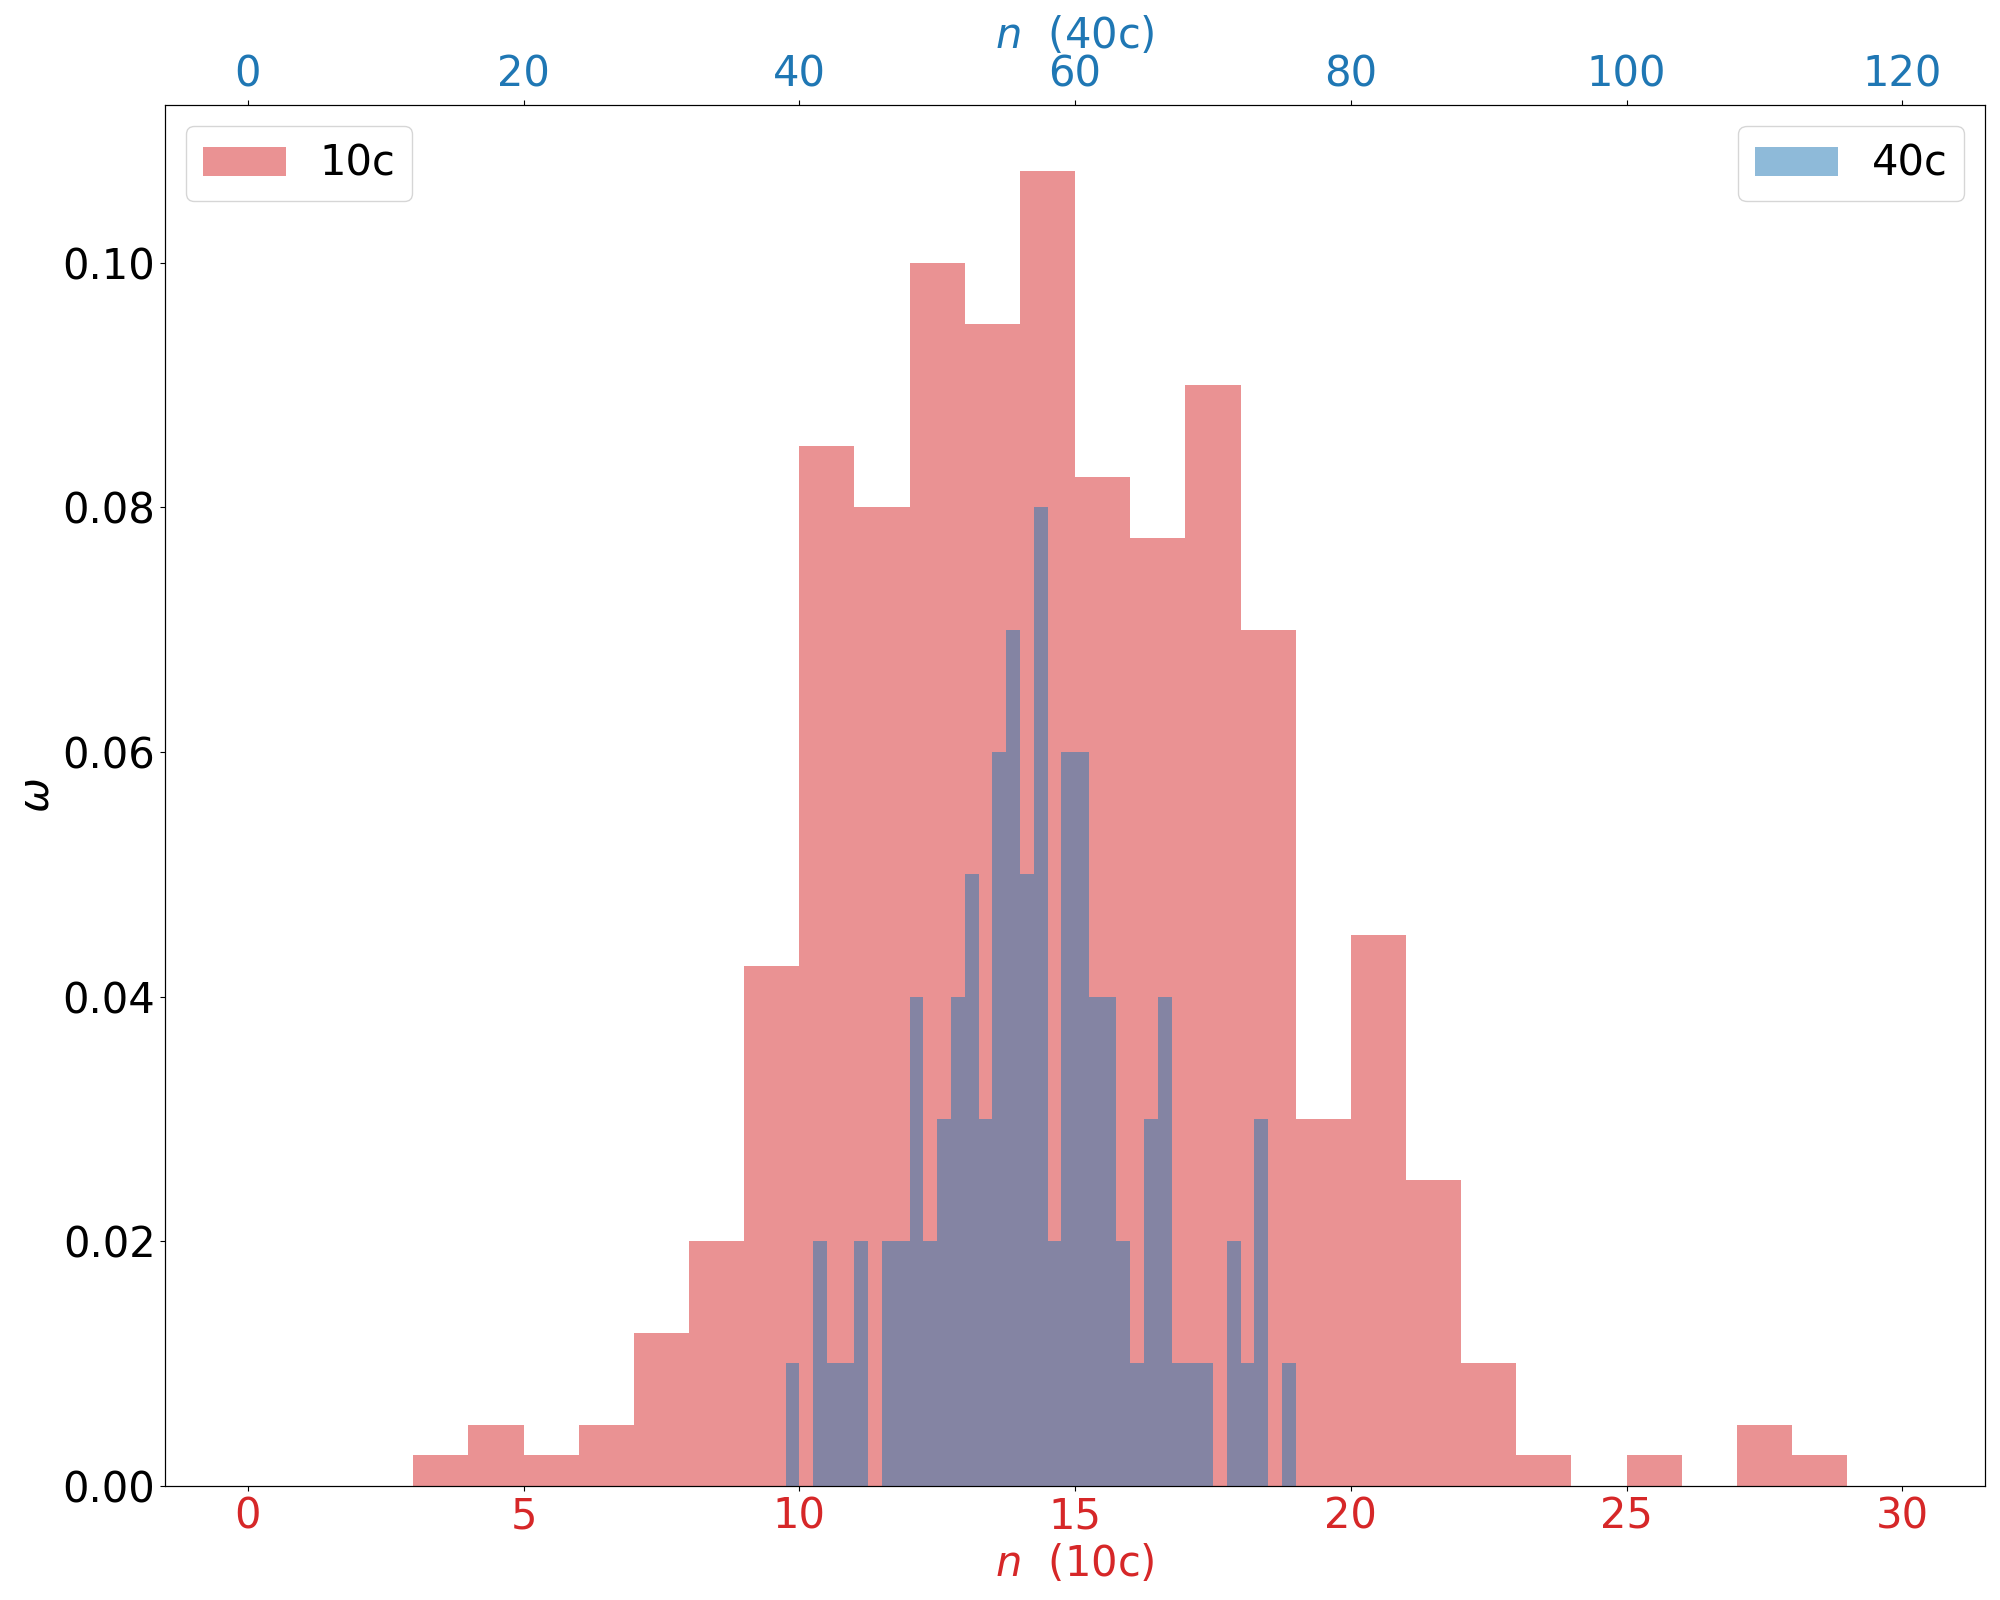
\includegraphics[scale=0.45]{histogram.png}
        \caption{Гистограммы для $t=10с$ и $t=40с$}
    \end{sidewaysfigure}
\end{document}
